\documentclass[border=10pt]{standalone}

\usepackage{tikz}
\usepackage{tikzsymbols}
\usetikzlibrary{calc,patterns,shapes.geometric}

\def\centerarc[#1](#2)(#3:#4:#5){\draw[#1] ($(#2)+({#5*cos(#3)},{#5*sin(#3)})$) arc (#3:#4:#5);}

\begin{document}
	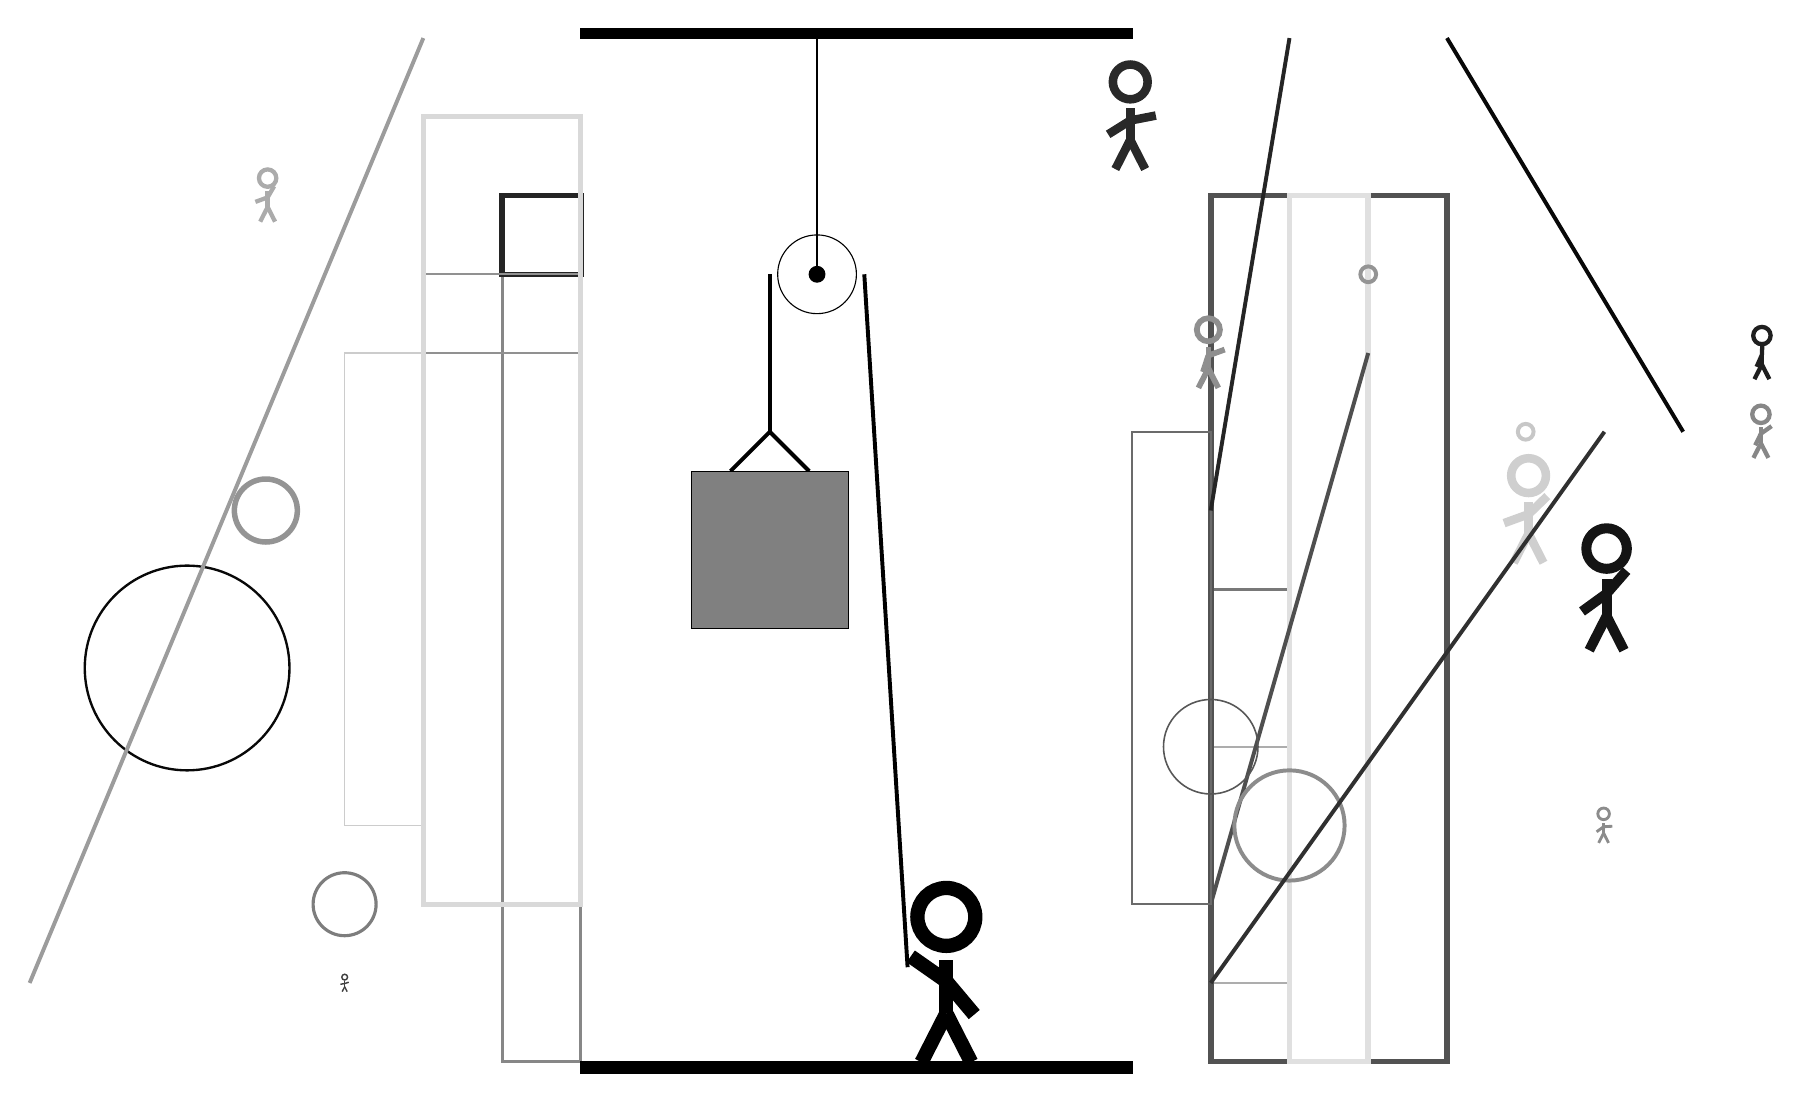
\begin{tikzpicture}
		%%%%% START %%%%%
		
		\draw[fill=black] (-2, 10) rectangle (5, 10.125);
		
		\draw [line width=0.3mm, color=black!97](-7, 2) circle (1.3);
		
		\draw[line width=0.4mm, color=black!47] (-3, 7) rectangle (-2, -3);
		\draw[line width=0.2mm, color=black!32] (7, 1) rectangle (6, -2);
		\node[line width=0.5mm, color=black!84] at (5, 9) {\Strichmaxerl[6][32][11]};
		
		\draw[line width=0.2mm, color=black!20] (-4, 0) rectangle (-5, 6);
		\draw[line width=0.4mm, color=black!53] (7, 3) rectangle (6, 3);
		\node[line width=0.2mm, color=black!75] at (-5, -2) {\Strichmaxerl[1][9][18]};
		\draw[line width=0.7mm, color=black!86] (-3, 7) rectangle (-2, 8);
		\draw [line width=0.7mm, color=black!42](-6, 4) circle (0.4);
		
		\draw[line width=0.7mm, color=black!68] (6, -3) rectangle (9, 8);
		\draw[line width=0.7mm, color=black!12] (7, 8) rectangle (8, -3);
		\node[line width=0.5mm, color=black!92] at (11, 3) {\Strichmaxerl[7][36][49]};
		\node[line width=0.2mm, color=black!33] at (-6, 8) {\Strichmaxerl[3][20][60]};
		\draw[line width=0.5mm, color=black!69](6, -1) -- (8, 6);
		\draw[line width=0.5mm, color=black!97](9, 10) -- (12, 5);
		\draw[line width=0.3mm, color=black!43] (-4, 6) rectangle (-2, 7);
		
		\draw[line width=0.3mm, color=black!69] (-2, 0) rectangle (-2, 7);
		\draw [line width=0.5mm, color=black!42](8, 7) circle (0.1);
		\draw[line width=0.2mm, color=black!58] (6, 5) rectangle (5, -1);
		\draw [line width=0.4mm, color=black!51](-5, -1) circle (0.4);
		\draw[line width=0.6mm, color=black!15] (-4, 9) rectangle (-2, -1);
		
		\draw [line width=0.2mm, color=black!66](6, 1) circle (0.6);
		\node[line width=0.7mm, color=black!44] at (6, 6) {\Strichmaxerl[4][72][20]};
		\draw[line width=0.5mm, color=black!39](-4, 10) -- (-9, -2);
		\draw [line width=0.5mm, color=black!22](10, 5) circle (0.1);
		\node[line width=0.3mm, color=black!19] at (10, 4) {\Strichmaxerl[6][20][44]};
		
		\node[line width=0.4mm, color=black!47] at (13, 5) {\Strichmaxerl[3][64][35]};
		\draw [line width=0.5mm, color=black!45](7, 0) circle (0.7);
		\node[line width=0.5mm, color=black!88] at (13, 6) {\Strichmaxerl[3][66][88]};
		\draw[line width=0.5mm, color=black!81](6, -2) -- (11, 5);
		\draw[line width=0.5mm, color=black!86](6, 4) -- (7, 10);
		\node[line width=0.3mm, color=black!45] at (11, 0) {\Strichmaxerl[2][36][3]};
		
		\draw (1, 7) circle (0.5);
		\draw[fill=black] (1, 7) circle (0.1);
		\draw (1, 10) -- (1, 7);
		
		\draw[line width=0.5mm] (-0.1, 4.5) -- (0.4, 5.0) -- (0.9, 4.5);
		\draw[fill=black!50] (-0.6, 4.5) rectangle (1.4, 2.5);
		
		\draw[line width=0.5mm] (0.4, 7) -- (0.4, 5.0);
		\centerarc[line width=0.5mm](1, 7)(0:180:0.6);
		\draw[line width=0.5mm](1.6, 7) -- (2.15, -1.8);
		
		\node at (2.6, -1.9) {\Strichmaxerl[10][-35][-50]};
		
		\draw[fill=black] (-2, -3) rectangle (5, -3.15);
		
		%%%%% END %%%%%
	\end{tikzpicture}
\end{document}